% !TEX TS-program = pdflatex
% !TEX encoding = UTF-8 Unicode

% This is a simple template for a LaTeX document using the "article" class.
% See "book", "report", "letter" for other types of document.

\documentclass[11pt]{scrreprt} % use larger type; default would be 10pt

\usepackage[utf8]{inputenc} % set input encoding (not needed with XeLaTeX)
\usepackage{german}
%%% Examples of Article customizations
% These packages are optional, depending whether you want the features they provide.
% See the LaTeX Companion or other references for full information.

%%% PAGE DIMENSIONS
\usepackage{geometry} % to change the page dimensions
\geometry{a4paper} % or letterpaper (US) or a5paper or....
% \geometry{margins=2in} % for example, change the margins to 2 inches all round
% \geometry{landscape} % set up the page for landscape
%   read geometry.pdf for detailed page layout information

\usepackage{graphicx} % support the \includegraphics command and options

% \usepackage[parfill]{parskip} % Activate to begin paragraphs with an empty line rather than an indent

%%% PACKAGES
\usepackage{booktabs} % for much better looking tables
\usepackage{array} % for better arrays (eg matrices) in maths
\usepackage{paralist} % very flexible & customisable lists (eg. enumerate/itemize, etc.)
\usepackage{verbatim} % adds environment for commenting out blocks of text & for better verbatim
\usepackage{subfig} % make it possible to include more than one captioned figure/table in a single float
\usepackage{german}
\usepackage{url}
\usepackage{hyperref}
\usepackage{amsfonts}
\usepackage{amsmath}
\usepackage{amsthm}
\usepackage{listings}
% These packages are all incorporated in the memoir class to one degree or another...

\usepackage{listings}
\usepackage{color}
\definecolor{lightgray}{rgb}{.9,.9,.9}
\definecolor{darkgray}{rgb}{.4,.4,.4}
\definecolor{purple}{rgb}{0.65, 0.12, 0.82}

\lstdefinelanguage{JavaScript}{
  keywords={typeof, new, true, false, catch, function, return, null, catch, switch, var, if, in, while, do, else, case, break},
  keywordstyle=\color{blue}\bfseries,
  ndkeywords={class, export, boolean, throw, implements, import, this},
  ndkeywordstyle=\color{darkgray}\bfseries,
  identifierstyle=\color{black},
  sensitive=false,
  comment=[l]{//},
  morecomment=[s]{/*}{*/},
  commentstyle=\color{purple}\ttfamily,
  stringstyle=\color{red}\ttfamily,
  morestring=[b]',
  morestring=[b]"
}

\lstset{
   language=JavaScript,
   backgroundcolor=\color{lightgray},
   extendedchars=true,
   basicstyle=\footnotesize\ttfamily,
   showstringspaces=false,
   showspaces=false,
   %numbers=left,
   numberstyle=\footnotesize,
   numbersep=9pt,
   tabsize=2,
   breaklines=true,
   showtabs=false,
   captionpos=b
}

%%% HEADERS & FOOTERS
\usepackage{fancyhdr} % This should be set AFTER setting up the page geometry
\pagestyle{fancy} % options: empty , plain , fancy
\renewcommand{\headrulewidth}{0pt} % customise the layout...
\lhead{}\chead{}\rhead{}
\lfoot{}\cfoot{\thepage}\rfoot{}

%%% SECTION TITLE APPEARANCE
\usepackage{sectsty}
\allsectionsfont{\sffamily\mdseries\upshape} % (See the fntguide.pdf for font help)
% (This matches ConTeXt defaults)

%%% ToC (table of contents) APPEARANCE
\usepackage[nottoc,notlof,notlot]{tocbibind} % Put the bibliography in the ToC
\usepackage[titles,subfigure]{tocloft} % Alter the style of the Table of Contents
\renewcommand{\cftsecfont}{\rmfamily\mdseries\upshape}
\renewcommand{\cftsecpagefont}{\rmfamily\mdseries\upshape} % No bold!

%%% END Article customizations

%%% The "real" document content comes below...

\theoremstyle{definition}
\newtheorem*{beisp}{Beispiel}
\newtheorem{definition}{Definition}
\newtheorem*{bemerkung}{Bemerkung}

\title{Systemtheorie und ein virtueller Trichter}
\subtitle{Seminar Syntax und Semantik \\ ZHAW, Zürich}
\author{Florian Lüthi\footnote{\url{luethifl@students.zhaw.ch}}}
%\date{ZHAW (Zürich), 5. Juni 2013} % Activate to display a given date or no date (if empty),
         % otherwise the current date is printed 

\begin{document}
\maketitle

\tableofcontents

\chapter{Einführung}

Diese Seminararbeit ist Teil des Seminars {\it{Syntax und Semantik}} an der ZHAW Zürich im Frühlingssemester 2013. Die Arbeit beschäftigt sich mit der allgemeinen Abgrenzung der Begriffe {\it Syntax} und {\it Semantik} in der Systemtheorie für physikalische Systeme. Das dazugehörige Programm {\tt VirtualFauceteering} soll die Thematik beispielhaft an einem einfachen System, bestehend aus einem Wasserhahn und einem Trichter, illustrieren.

{\tt VirtualFauceteering} wie auch dieses Dokument können von \url{https://github.com/foyan/VirtualFaucet} bezogen werden.

Der Autor bedankt sich bei den Dozenten Albert Heuberger und Beat Seeliger für die Kursführung.

\chapter{Syntax und Semantik in der Systemtheorie}

\chapter{Illustrierendes System}

\section{Setup}

Um die Wechselwirkung von Syntax und Semantik an einem physikalischen System illustrieren und simulieren zu können, wird die folgende Versuchsanordnung angenommen. Man beachte, dass wir uns mit unserer Anordnung im Flächenland befinden; dies bedeutet, dass  alle involvierten Volumina zweidimensional als Flächen berechnet werden, in der Realität aber Rotationskörper wären.

\begin{itemize}
\item Ein Wasserhahn, der mit konstantem Ausflussvolumen entweder läuft oder nicht:
\[
	\Delta V_{\text{out}} \in \{ 0, 200 \}
\]
\item Ein Trichter, dessen Wand durch die Radiusfunktion (abhängig von der Höhe $h$)
\[
	r(h) = \begin{cases}
		4 & (h = 0) \\
		r'(h) + 4 & (h > 0)
	\end{cases}
\]
mit 
\[
	r' : \mathbb{R} \rightarrow \mathbb{R}
\]
beschrieben wird und der eine untere Trichteröffnung von $r(0) = 4$ besitzt.

Da das Volumen des Wassers innerhalb des Trichters bei bekannter Pegelhöhe der Integralfunktion
\[
V(h) = 2\cdot \int\limits_{0}^{h} r(x) dx
\]
entspricht, ist die Funktion der Pegelhöhe die Lösung $h$ der folgenden Gleichung:
\[
\int\limits_{0}^{h} r(x) dx - \frac 1 2 \cdot V_h = 0
\]

Die Berechnung der Ausflussgeschwindigkeit $v$ des Wassers aus dem Trichter ergibt sich gemäss dem Torricellischen Gesetz \cite{wiki:ausflussgeschwindigkeit}:
\[
v = \sqrt{2gh}
\]

\item Eine Messvorrichtung, welche die momentane Ausflussgeschwindigkeit messen kann.

\end{itemize}

\section{Ermittlung der Ausgabe-Semantik}

Bei gegebener Eingabe und bekannter Syntax ist die Ermittlung der Ausgabe trivial, denn sie entspricht direkt der gemessenen Ausflussgeschwindigkeit.

\section{Ermittlung der Eingabe-Semantik}

Bei gegebener Ausgabe und bekannter Syntax gestaltet sich die Ermittlung der Eingabe folgendermassen:

\begin{enumerate}
\item Ermittle die Pegelhöhe $h$ innerhalb des Trichters mit der Umkehrung des Torricellischen Gesetzes:
\[
	h(t) = \frac {v^2(t)}{2\cdot g}
\]
\item Ermittle das Volumen des sich momentan im Trichter befindenden Wassers durch Integration über $r(h)$:
\[
	V(t) = 2\cdot \int\limits_0^{h(t)} r(x) dx
\]
sowie das ausgeflossene Volumen durch
\[
	\Delta V_\text{out}(t) = 2\cdot v(t) \cdot r(0) \cdot \Delta t.
\]
\item Ermittle die totale Änderung des Volumens durch
\[
	\Delta V(t) = V_t - V_{t-\Delta t}
\]
sowie daraus folgend das vom Wasserhahn in den Trichter geflossene Volumen durch
\[
	\Delta V_\text{in}(t) = \Delta V(t) + \Delta V_\text{out}(t).
\]
\end{enumerate}

\section{Ermittlung der Syntax}

Dies ist der schwierigste Teil. Bei gegebener Eingabe $\Delta V_\text{in}(t)$ und gegebenen Ausgaben $v(t)$ und $\Delta V_\text{out}(t)$ (sowie daraus abgeleitet der Höhe $h(t) = \frac {v^2(t)}{2\cdot g}$) ergeben sich die Messpunkte $\tilde r$ durch
\[
	\tilde r(h(t)) = \frac {\Delta V_t}{2 \cdot \Delta h_t} = \frac {\Delta V_\text{in}(t)-\Delta V_\text{out}(t)} {2 \cdot h(t) - h(t-\Delta t)}.
\]

Die notwendige analytische Beschreibung der Syntax kann in beschränktem Masse durch Regression erreicht werden.

\chapter{Bemerkungen zur Implementation}

\section{Umgebung}

Das verwendete Programmierumfeld ist HTML und JavaScript. Dadurch ist gewährleistet, dass das Programm auf allen möglichen Plattformen lauffähig ist. Ausserdem verlangt die sinnvolle Umsetzung der Thematik ein relativ stark ausgebautes User Interface zur Illustration. Dies ist mit HTML relativ einfach und mit geringem Aufwand möglich.

Alternativen wurden bewusst nicht evaluiert.

\section{Libraries}

Die eingesetzten JavaScript-Libraries sind:
\begin{itemize}
\item {\tt jQuery} \cite{lib:jquery} zur Vereinfachung einiger DOM-Operationen sowie wegen einiger nützlicher Routinen zur funktionialen Programmierung wie {\tt \$.map()} und {\tt \$.grep()},
\item {\tt gRaphaël} \cite{lib:graphael} für die Plots,
\item {\tt knockout.js} \cite{lib:knockout} für das einfache Binding von Modell und User Interface.
\end{itemize}

\section{Architektur}

Die Architektur des Programms ist in Abbildung \ref{architecture} skizziert. In den folgenden Abschnitten werden die Komponenten kurz erläutert und wo notwendig, interessant und/oder sinnvoll Kommentare zum Code abgegeben.

\begin{figure}
\caption{Architektur}
\label{architecture}
\begin{center}
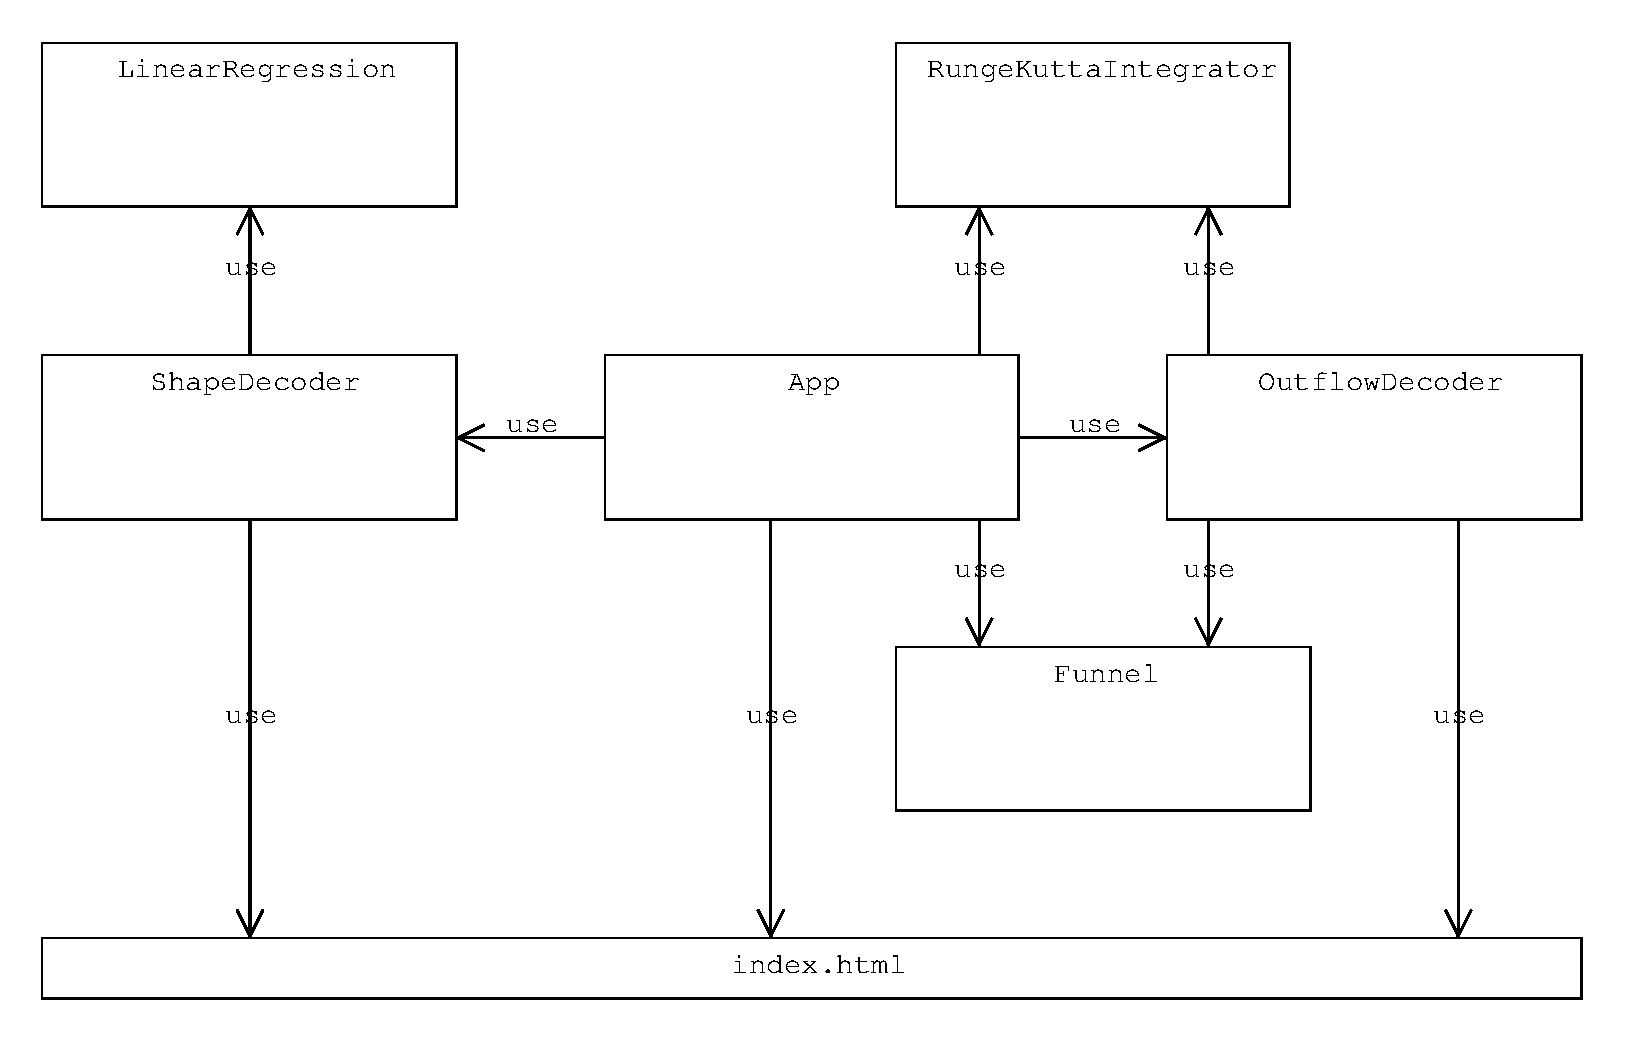
\includegraphics[scale=0.5]{biltli/architecture.pdf}
\end{center}
\end{figure}


\subsection{{\tt App}}

Diese Klasse hält den momentanen Zustand des Modells. Ausserdem ist sie verantwortlich für das Zeichnen des Trichters sowie weiter Teile des User Interfaces.

\subsection{{\tt Funnel}}

Diese Klasse definiert den Trichter. Sie besteht mehr oder weniger aus der Methode {\tt radius()}, welche den Radius des Trichters in Abhängigkeit von der Höhe zurückgibt:

\begin{lstlisting}
this.radius = function (h) {
	if (h <= 1) {
		return 4;
	}
	return 4 + self.r_h()(h-1);
}
\end{lstlisting}

{\tt r\_h} ist ein {\tt knockout}-Observable, das die benutzerdefinierbare innere Funktion speichert.

\subsection{{\tt OutflowDecoder}}

Diese Klasse repräsentiert den Decoder, welcher den Ausfluss aus dem Trichter analysiert und daraus den Einfluss wieder herstellt. Die Analyse passiert folgendermassen:

\begin{lstlisting}
this.report = function (x, v) {
	
	var h = v > 0 ? v * v / 2.0 / 9.81 : 0;
	var V = self.integrator.integrate(0, 0, self.funnel.radius, h) * 2;

	var dV = V - self.prevV;
	var dVo = self.prevv * self.funnel.radius(0) * 2 * dt;
	var dVi = dV + dVo;
		
	/* [...] */
		
	var bit = dVi > 90.0;
	self.prevV = V;
	self.prevv = v;

	/* [...] */
}
\end{lstlisting}

Im Falle von Semantik in Form von Text muss noch der Text aus der binären Repräsentation wiederhergestellt werden:

\begin{lstlisting}
this.report = function (x, v) {
	
	/* [...] */

	self.currentByte = ((self.currentByte << 1) + bit) & 255;
	var ch = self.isPrintable(self.currentByte) ? String.fromCharCode(self.currentByte) : "\u00A0";
	var newText = self.plainText[x % 8]() + ch;
	if (newText.length > 100) {
		newText = newText.substr(newText.length - 100, 100);
	}

	/* [...] */

	self.plainText[x % 8](newText);
}
\end{lstlisting}

{\tt plainText[]} enthält acht {\tt knockout}-Observables mit Text. Dies ist nötig, weil der Decoder nicht weiss, in welchem Zeitschritt die Übertragung begonnen hat, und es deswegen acht verschiedene Möglichkeiten gibt, den Bitstrom zu Bytes zusammenzusetzen.

Trotzdem macht natürlich nur eine dieser acht Textsequenzen Sinn. Welche das ist, versucht die eingebaute Gibberish Detection zu erkennen:

\begin{lstlisting}
this.report = function (x, v) {
	
	/* [...] */
	for (var i = 0; i < 8; i++) {
		self.gibberishFactors[i] *= 0.99;
	}

	self.gibberishFactors[x % 8] += self.isGibberish(self.currentByte) ? 0.0 : 0.125;
		
	var minIndex = self.minGibberishIndex();
	var minGibberish = self.gibberishFactors[minIndex];
	for (var i = 0; i < 8; i++) {
		if (self.gibberishFactors[i] > minGibberish) {
			minGibberish = self.gibberishFactors[i];
			minIndex = i;
		}
	}
	self.minGibberishIndex(minIndex);

	/* [...] */

}
\end{lstlisting}

Die Gibberish Detection hält für jede der acht Sequenzen einem numerischen Wert vor, der sich um 0.125 erhöht, wenn an die Sequenz ein druckbares Zeichen angefügt wird. Vorgängig wird jeweils der Wert für alle Sequenzen um ein Prozent verringert -- dies führt dazu, dass neue Übertragungen einigermassen unabhängig von der jeweils vorhergehenden analysiert werden können.

Die verwendeten Werte sind empirisch, scheinen sich aber im Praxiseinsatz zu bewähren.

\subsection{{\tt ShapeDecoder}}

Diese Klasse hat die Aufgabe, aus gegebener Eingabe und gegebener Ausgabe die Syntax wiederherzustellen -- sprich die Radiusfunktion des Trichters.

Dies tut sie, indem sie lineare Regression für verschiedene Funktions-Skelette durchführen lässt und dann dasjenige mit dem kleinsten normierten Residuum selektiert:

\begin{lstlisting}
this.guess = function () {
	var reg = new LinearRegression();
		
	var minR = 99999999;
	var minRguess = -1;
	for (var i = 0; i < self.guesses.length; i++) {
		var res = reg.calculate(self.x, self.yr, self.guesses[i].mode);
		self.guesses[i].func = res.func;
		self.guesses[i].x(res.x);
		self.guesses[i].residual(res.residual);
		self.guesses[i].isLeader(false);
			
		if (res.residual < minR) {
			minRguess = i;
			minR = res.residual;
		}
	}
		
	if (minRguess != -1) {
		self.guesses[minRguess].isLeader(true);
	}
}

\end{lstlisting}

\subsection{{\tt LinearRegression}}

Diese Klasse nähert eine Reihe von Messpunkten durch eine Funktion mit linearen Koeffizienten an. Das tut sie, indem sie aus den Messpunkten $(u_1, v_1), (u_2, v_2), \dots, (u_n, v_n)$ sowie den unbekannten Koeffizienten $x^* = \{x^*_1, x^*_2, \dots\}$ das Ausgleichsproblem

\[
||Ax^* - b||_2 = \min_{x \in \mathbb{R}^n} ||Ax - b||_2
\]

%
%\[
%A^TAx^* = A^Tb
%\]
%mit
%\[
%b = \{v_1, v_2, \dots\}
%\] und \[
%A = \begin{bmatrix}
%f_{1}(u_1) & f_{2}(u_1) & \dots & f_m(u_1) \\
%f_1(u_2) & f_2(u_2) & \dots & f_m(u_2) \\
%\vdots & \vdots & \ddots & \vdots \\
%f_1(u_n) & f_2(u_n) & \dots & f_m(u_n)
%\end{bmatrix}
%\]

ableitet \cite{massjung}. Durch eine $QR$-Zerlegung von $A$ mittels Householder-Transformation (\cite{wiki:householder}) kann das äquivalente Ausgleichsproblem 

\[
||QAx^* - Qb||_2 = \min_{x \in \mathbb{R}^n} ||Ax - b||_2
\]

einfach gelöst werden, weil $R$ eine obere Dreiecksgestalt hat. Die Residuen werden von den durch die Überdeterminierung überflüssigen Komponenten von $Qb$ repräsentiert.

Die implementierte Methode verdeutlicht das Vorgehen:

\begin{lstlisting}
this.calculate = function (u, v, mode) {
	
	var vs = [];
		
	var A = mode.getA(u);
	var R = self.getR(A, vs);
	var b = mode.getB(v);
	var Qb = self.transformB(b, vs, mode.coeffs);
	var x = self.solve(Qb, R, mode.coeffs);
	var res = self.getResidual(Qb, x);
				
	return {
		x: x,
		func: mode.getFunction(x),
		residual: res
	};
		
}
\end{lstlisting}

\subsection{{\tt RungeKuttaIntegrator}}

Zur Berechnung der anfallenden Integrale implementiert die Klasse {\tt RungeKuttaIntegrator} das Bogacki-Shampine-Verfahren (\cite{wiki:bogackiShampine}). Es handelt sich dabei um ein Verfahren aus der Familie der expliziten Runge-Kutta-Verfahren, welches die Ordnung 3 hat und zur automatischen Steuerung der Schrittweite $h$ ein eingebettetes Verfahren der Ordnung 2 aufweist.

Derlei Verfahren mit Schrittweitensteuerung sind im Allgemeinen massiv effizienter als Verfahren mit fester Schrittweite, haben allerdings das Problem, dass die genaue Berechnung eines Integrals zwischen zwei Grenzen nicht möglich ist.

Aus diesem Grund kombiniert diese Klasse die beiden Verfahren: Es wird mittels Bogacki-Shampine möglichst nahe an die obere Grenze heranintegriert. Danach wird für das restliche Intervall das klassische Runge-Kutta-4-Verfahren herangezogen:

\begin{lstlisting}
this.integrate = function (y0, t0, y, tend) {
	var r = self.bogackiShampine(y0, t0, y, tend, 0.01, 0.00001);
	return self.rungeKutta4(r.ym1, r.tm1, y, tend).y;
}
\end{lstlisting}

Die Berechnung der Pegelhöhe $h$ als Nullstelle der nichtlinearen Funktion $\int_0^h r(x) dx - V_h$ verlangt eigentlich nach einem passenden Verfahren. Dies ist allerdings sehr ineffizient, da die mehrfache Auswertung der Integralfunktion sehr ineffizient ist.

Allerdings wissen wir, dass die Funktion  $f(h) = \int_0^h r(x) dx$ (wie jede Integralfunktion) monoton steigend sein muss. Ausserdem wissen wir, dass sie sogar streng monoton steigend sein muss -- ansonsten wäre r(x) an einer Stelle $x  \ne 0$ gleich null, was nicht möglich ist (denn dann wäre der Trichter nicht mehr durchlässig).

\chapter{Schlussfolgerungen}

\bibliography{biblio}
\bibliographystyle{plain}


\end{document}
